\section{Nebulas Rank}
\label{sec:rank}

\subsection{Overview of Nebulas Rank} \label{subsec:value}
Currently the Blockchain technology and community have grown into a large scale ecosystem. However, people's perception of Blockchain world is still relatively flat; there is no reasonable way to evaluate the value of an entity (such as user address) on the blockchain yet. Therefore, we try to come up with a universal measure of value. By exploring and utilizing activities on chain, we create \textbf{Nebulas Rank} through which the value of each entity (user address) is able to be quantified. \textbf{Nebulas Rank} is designed to:\begin{itemize}
	\item serve as a native measure of value and a core algorithm for many fundamental scenarios, such as consensus algorithm (see \refsec{sec:pod}), DIP (see \refsec{sec:dip}) and Blockchain search engine (see \refsec{sec:search}), etc;
	\item inspire diversified measures of value and deeper insights into the blockchain ecosystem, so as to better guide business decisions and research activities.
\end{itemize}
Based on the goals above, we define the measure of value of \textbf{Nebulas Rank} from three dimensions:
\begin{itemize}
	\item Liquidity, the frequency and scale of transactions, is the first dimension that \textbf{Nebulas Rank} measures. Finance essentially is the social activities which optimize social resources via capital liquidity and promote economic development. Blockchain establishes a network of value. More transactions and larger transaction scale produce better liquidity, and better liquidity further increases transactions and transaction scale, forming a complete mechanism of positive feedback.
	\item Propagation, the scope and depth of asset liquidity, is the second dimension that \textbf{Nebulas Rank} measures. In social network, the propagation property, i.e. speed, scope and depth of information transmission, is a key index indicating network quality and user growth. We see the same pattern in the Blockchain world. Powerful propagation means wider and deeper asset liquidity, which improves the quality and scale of assets in the Blockchain world.
	\item Interoperability is the third dimension that \textbf{Nebulas Rank} measures. During the early stage of Internet, there were just simple websites and isolated information. Now information on different platforms can be forwarded on the network, and isolated data silos are gradually being broken. This tendency could be understood as a process of recognizing information from higher dimensional perspective. We believe that Blockchain world also follows a similar pattern, whose development will be faster. There will be more information of users' assets, smart contracts and DApp. And also, there will be more frequent interactions among them. Therefore, better interoperability will become more important.
\end{itemize}

We choose transaction records on chain as source data for \textbf{Nebulas Rank}. That is because the "trajectory" in Blockchain world is more clear and trustworthy than that in the real world. Transaction data such as transfers and callings of "smart contracts" are all recorded on chain. But it is not trivial to design rank algorithm for Blockchain transaction data, since the transactions in Blockchain world are naturally anonymous and bear larger data scale than that in the real world. Three major properties for \textbf{Nebulas Rank} are described below:
\begin{itemize}
	\item Truthful. An entity must pay reasonable costs to improve its ranking, which assures that the algorithm can identify trusted valuable users. On one hand, in scenarios like consensus algorithm and DIP, truthful ranking encourages users to contribute truthfully in order to realize positive feedback. On the other hand, truthful result provides meaningful hierarchy representation of all users, which will be more helpful for decision makers;
	\item Computable. As a fundamental field, the result of \textbf{Nebulas Rank} should be accessible instantly and thus requires low computational complexity;
	\item Reproducible. As required by scenarios such as consensus algorithm and DIP, the computing result of \textbf{Nebulas Rank} should be identical at any client.
\end{itemize}

Next we design the basic framework of \textbf{Nebulas Rank}. First, transaction records are represented in the form of graph. In the transaction graph (entity graph), every node is mapped to one entity, and each edge represents the transfer between two entities\cite{Tschorsch2015}. Transaction graph embodies the fact that money transfer among users leads to assets flowing, which helps to represent the concepts of liquidity and propagation defined before. Meanwhile, the form of graph can clearly display the interoperability among contracts. With the derived transaction graph, we rank nodes by their network centrality. In the scenario of \textbf{Nebulas Rank}, LeaderRank\cite{Chen2013}\cite{Li2014} is a more reasonable measurement and outperforms PageRank of Google and NCDAwareRank of NEM\cite{nem}.

\subsection{Transaction Graph} \label{subsec:txg}
This subsection introduces how to derive transaction graph from transaction history.

First, for any time $t_0$, we take all \textbf{effective} transactions among individual addresses during $[t_0- T, t_0]$ (generally $T$ is a constant of one month), where every transaction can be represented as a 4-tuple $(s,r,a,t)$, with $s$ as the source address, $r$ as the target address, $a$ as the transfer amount and $t$ as the block time. We define a transaction to be \textbf{effective} iff $a>0$ and $s \neq t$. Thus all \textbf{effective} transactions during $[t_0- T, t_0]$ can be represented by a set of 4-tuples:

\begin{align}
\Theta(t_0) = \{(s, r, a, t)\ |\ t_0 - T \le t \le t_0\ \land \ a > 0 \land s \neq t \}	
\end{align}

Then based on $\Theta(t_0)$, construct a directed weighted simple graph $G=(V,E, W)$, where node set, edge set and edge weights are denoted by $V$, $E$ and $W$ respectively. Every node in $V$ represents an individual account's address, and each edge in $E$ represents the transfer intensity between two addresses. Edges are directed and are assigned with weight $w_e$ aggregating top $K$ amounts of all related transactions:
\begin{align}\label{formula:edgeweight}
w_e = \sum_{i=1}^K a_i,\ s.t.\ a_i \in A
\end{align}
$A$ is an ordered set consisting of amounts of all transactions in $\Theta(t_0)$:
\begin{align}
A = \{a_i\ |\ a_i \in \Theta(t_0) \land (a_i \ge a_j, \forall i \le j) \}
\end{align}

Additionally, let $N = |V|$,$M = |E|$, where $|.|$ is the cardinal number of a set. For simplicity, every node is represented by an integer between $1$ and $N$.

\begin{figure}[h]
\centering
	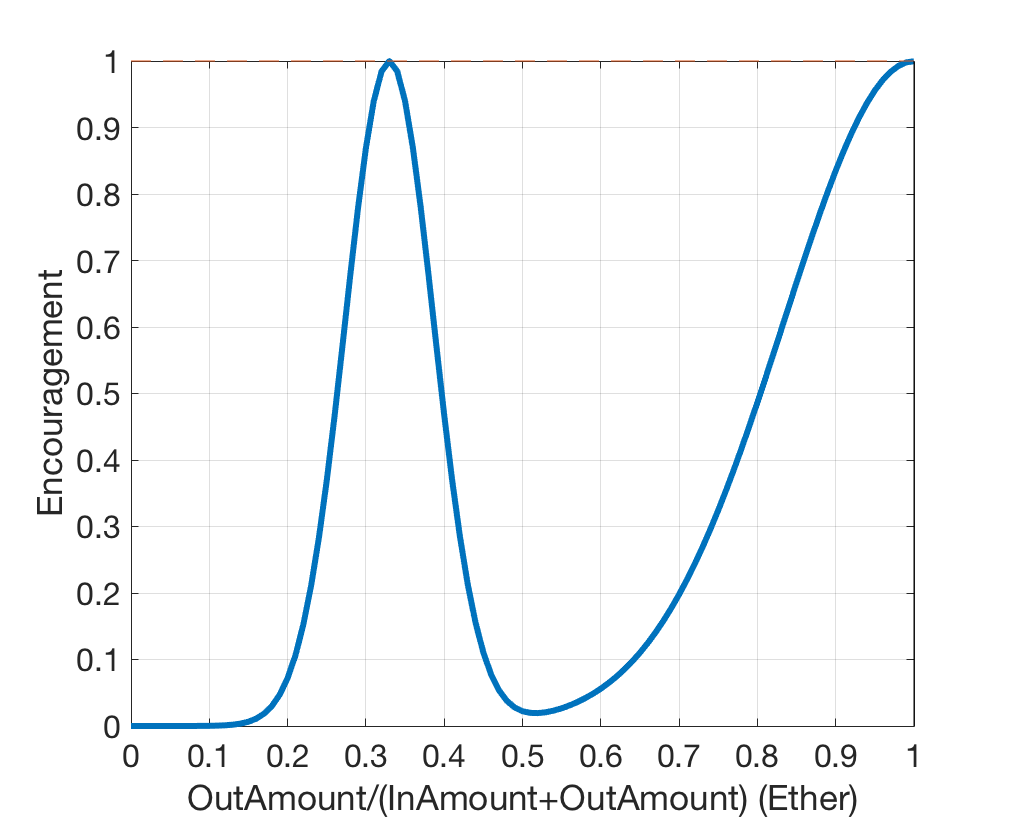
\includegraphics[width=0.55\textwidth]{figs/encouragement_en.png}
	\caption{Encouragement Function}\label{fig:encouragement}
\end{figure}

Then, for each node, according to its in-transfers and out-transfers during $[t_0\ −\ T,\ t_0]$, compute the "coinage" and denote it by $C_v$; based on the total transfer amount and using the "encouragement function" shown in \reffig{fig:encouragement}, compute the encouragement value and denote it by $E_v$\footnote{Encouragement function can be represented as a linear combination of two normal distributions, which outputs peak value when the money transferred out is zero or of some ratio of the amount transferred in.}; use $C_v$ and $E_v$ of the target nodes to reduce the edges' weight.

Finally, take the largest weakly connected component of the whole graph, only remaining nodes belonging to this component. The deleted nodes are assigned with lowest importance score by default.

The graph derivation described above contributes to the "truthful" property defined at \refsec{subsec:value}, the evidence of which is shown in \refsec{subsec:robust}.

Using the method described herein, the transaction graph, wherein $T$ is 30 days and $K=2$, is created on the basis of transaction data in the main chain of Ethereum, from block \#3629091(roughly on May 1st, 2017) to block \#3800775(roughly on May 31st, 2017). Its visualization is shown as \reffig{fig:wgc}. , and all nodes are resized by their degree. It could be observed that some famous exchanges usually interacts with more accounts than others. Besides, the identities of some addresses who contribute a lot transactions still remains unknown. 

\begin{figure}[htbp]
	\centering
	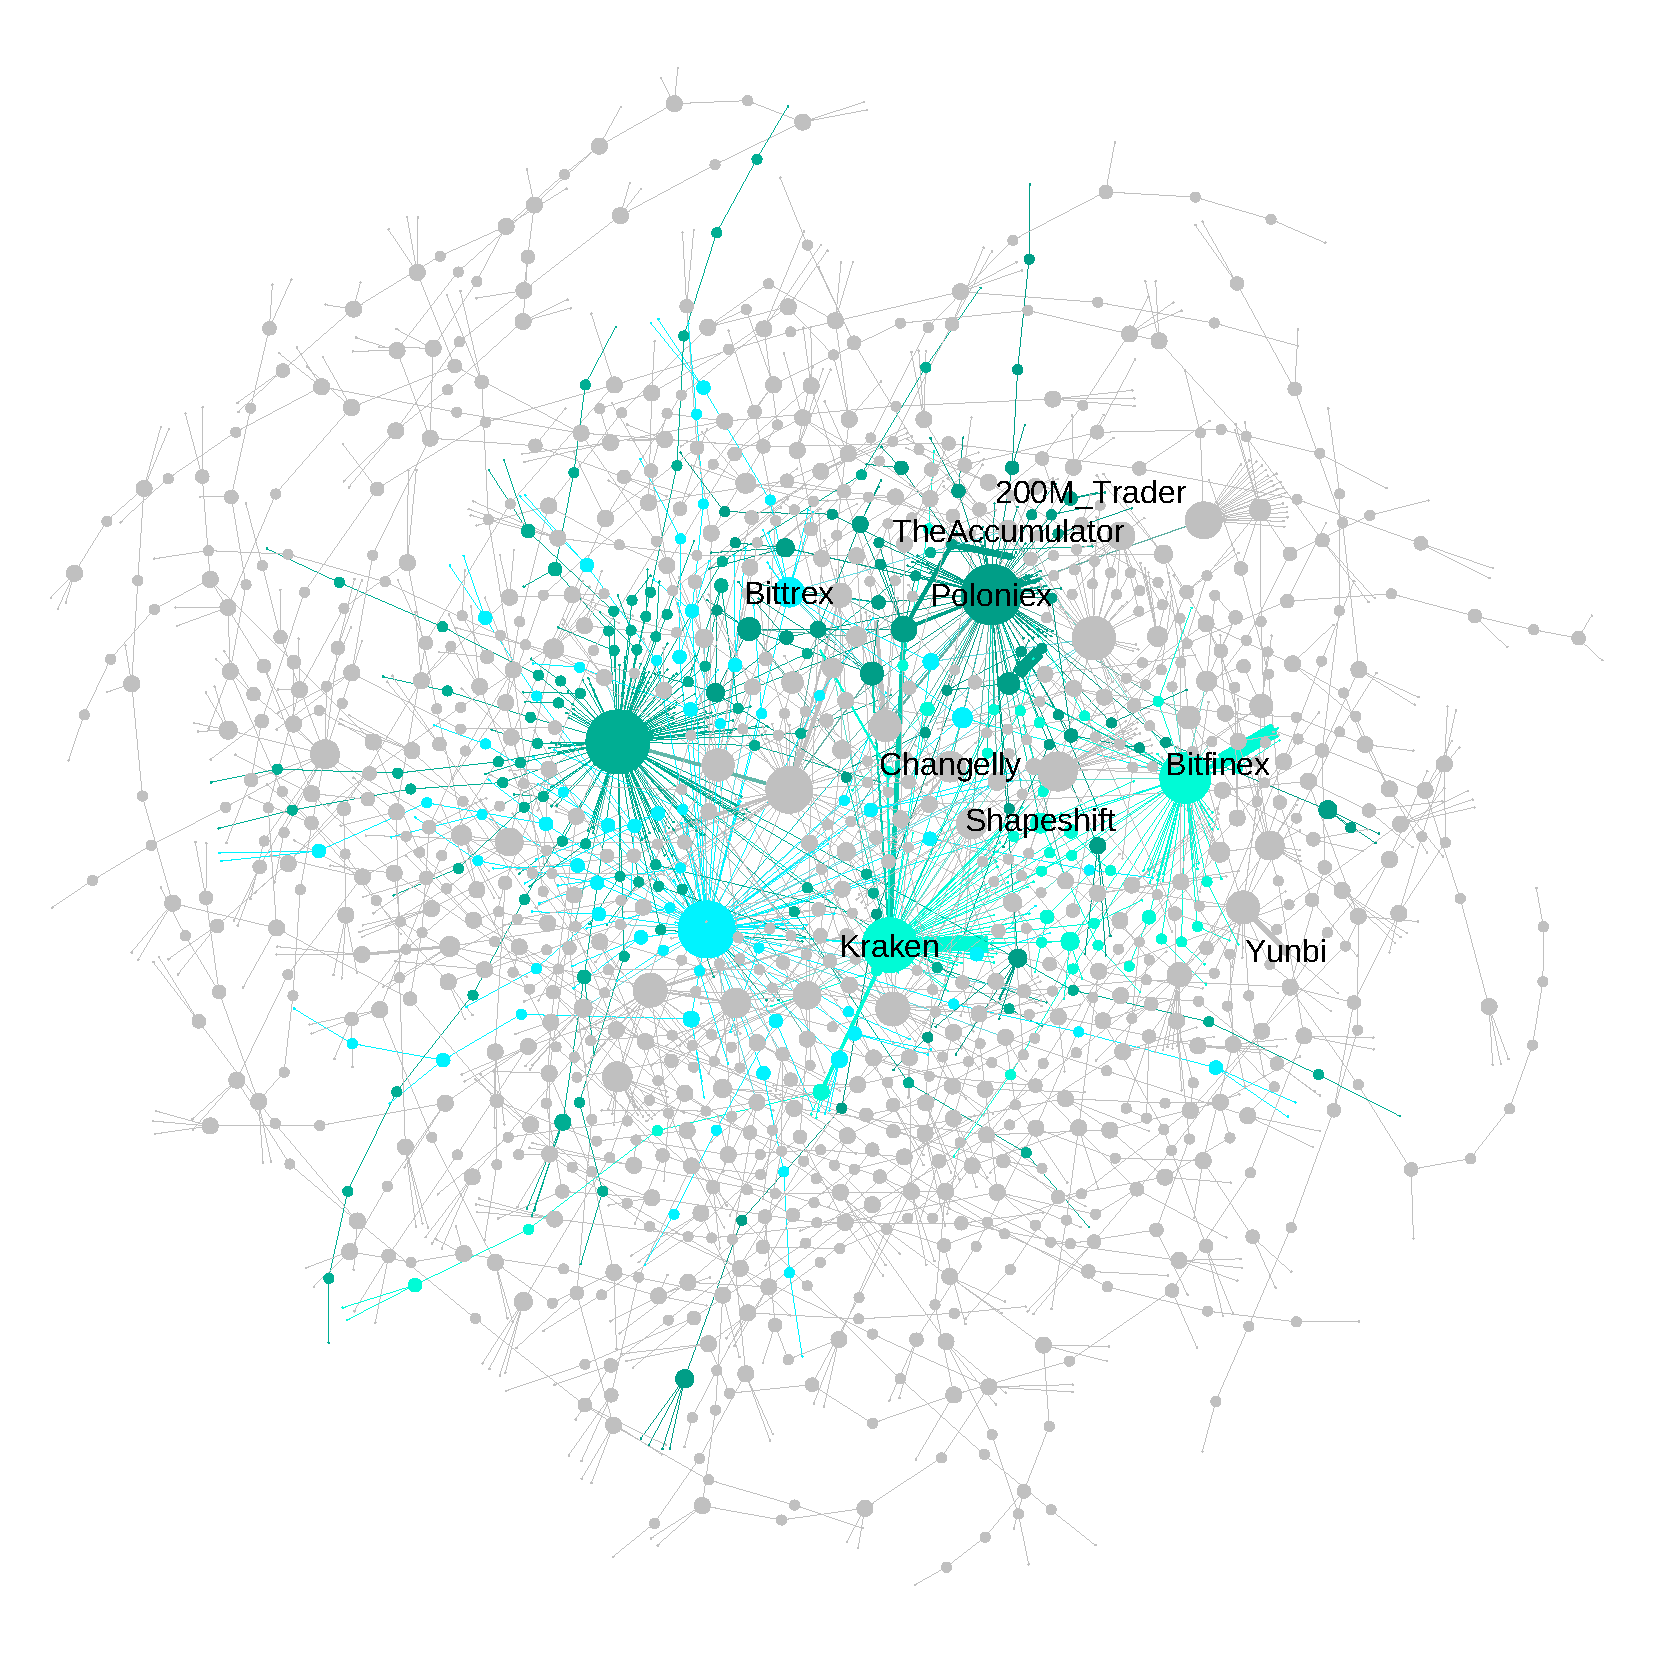
\includegraphics[width=0.85\textwidth]{figs/wgc1.png}
	\caption{Transaction Graph (Partly) Visulazation. \small{Large transaction scale (capital transfer) in the address means high in-and-out degree in the node, represented by large diameter in the figure. Some nodes are labeled by tags in Etherscan\cite{etherscan}}  }\label{fig:wgc}
\end{figure}

\subsection{Ranking Algorithm} \label{subsec:leaderrank}
This subsection introduces how to rank nodes by their importance in the derived transaction graph.

We adopt LeaderRank\cite{Chen2013}\cite{Li2014} as the main algorithm. First, add a ground node with index $0$ into the transaction graph. Then establish double link between the ground node $0$ and every other node $i$ ($1 \leq i \leq N$), weighting by the following formula:
\begin{align}\label{formula:weight1}
w_{i,0} = \alpha( max\{ \sum_{w_{j,i} \neq 0} w_{j,i} - \sum_{w_{i,j} \neq 0} w_{i,j} , 0\} + \lambda C ), \forall i \in [1,N]	
\end{align}
\begin{align}\label{formula:weight2} 
w_{0,n}	= \beta ( \sum_{w_{n,m} \neq 0} w_{n,m} + \mu C), \forall i \in [1,N]
\end{align}
$C$ is the median of set $\{w_{i,j} | w_{i,j} \neq 0, 0\leq i,j \leq N\}$, and $\alpha, \beta, \mu, \lambda$ are parameters. 

The weighting scheme can be understood as that, nodes with more in-degree receive more in-link from the ground node; nodes with more absolute income, i.e. in-degree minus out-degree, outputs stronger link into the ground node. 

The computing process of LeaderRank is similar with that of PageRank, which could be understood as computing the convergence state of a Markov process. What is different is that, after adding the ground node, it does not need to consider the damping factor of PageRank\cite{Brin2010}\cite{page1999pagerank} anymore. That is, after constructing matrix $H$ according to formula (\ref{formula:matrix}), the computing process is iterated until convergence, as formula (\ref{formula:iteration}) shows, with initial settings defined by formula (\ref{formula:init}). Finally the rank score of ground node is distributed evenly to every other node, which yields the final score for every node.
\begin{align} \label{formula:iteration}
	P^{t+1} = H \times P^{t}; P^1=[\frac{1}{N}, \frac{1}{N}, \dots, \frac{1}{N}, 0]^T
\end{align}
\begin{align} \label{formula:matrix}
	h_{ij} = \frac{w_{(j,i)}}{\sum_k w_{(j,k)}}
\end{align}
\begin{align} \label{formula:init}
\forall v \in V, P^*_v \leftarrow P^*_v + \frac{P^*_{\mathcal{G}}}{N}
\end{align}

We suppose that LeaderRank can satisfy the measure of value and algorithm property defined in \refsec{subsec:value}.
\begin{itemize}
	\item The result of LeaderRank can be understood as the flux on each node in the dynamic equilibrium of money exchange network, which matches \textbf{Nebulas Rank}'s measure of value: "liquidity", "propagation" and "interoperability";
	\item The weighing scheme defined by formula (\ref{formula:weight2}) and (\ref{formula:weight1}) makes it more difficult to attack (see discussion in \refsec{subsec:robust}), which satisfies "truthful" property;
	\item LeaderRank can be computed by power iteration. Since the network is very sparse, the complexity of matrix computation should not be high, which satisfies the properties of "computable" and "reproducible".
\end{itemize}


\subsection{Manipulation Resistance}\label{subsec:robust}
Truthfulness, i.e. the ability of resisting manipulation, is the most significant and challenging goal of \textbf{Nebulas Rank}. Some manipulation methods are as follows:
\begin{enumerate}
	\item Loop transfer. The attacker transfers along a loop topology, which allows the same money flow over same edges repeatedly. By this means, the attacker hopes to raise the weight of related edges;
	\item Transfer to random addresses, so that the out-degree of sybil node is increased, and the propagation of fund is increased as well;
	\item Form an independent network component with addresses controlled by the attacker. So the attacker can pretend to be a central node;
	\item Interact with authoritative Exchange service addresses frequently, i.e. transfer the same money in and out an authoritative Exchange service address repeatedly, so that the attacker can acquire better structural position in the network.
\end{enumerate}

\textbf{Nebulas Rank} mitigates manipulation through the following mechanism:
\begin{itemize}
	\item Owing to sliding windows of $T$ blocks, the attacker cannot increase its rank in short term;
	\item Since the edge weight is decided by the related transactions with highest amount , transferring along a loop topology cannot increase edges' weight unlimitedly. Meanwhile, according to the sampled data in \refsec{subsec:txg}, $91\%$ of edges correspond to less than 2 transactions respectively. Thus $K=2$ is a reasonable choice to remain the intensity information on edges while being resistance to loop transfer;
	\item In order to have higher "coinage", the user needs to let money stay in their address for a while, which slows down the attacking speed;
	\item In order to get the maximum "encouragement value", as is shown in \reffig{fig:encouragement}, the account needs to keep all income or transfer out only a small ratio of it. So when forging money flow, the attacker will get a rapid decrease in its deposit;
	\item Because only the giant component is selected, other independent components including the forged one will be filtered out as noise. According to the sampled data in \refsec{subsec:txg}, there are $453,285$ nodes and $970,577$ edges, with $1,169$ components. In the biggest component, there are $449,746$ nodes, accounting for $99.2\%$ of the total number. In the second biggest component, there are just $133$ nodes, only accounting for $0.03\%$. Thus taking the giant component can remain normal part of network as much as possible while filtering noise part out;
	\item Compared with webpage ranking algorithms such as PageRank and NCDawareRank\cite{Nikolakopoulos2013}, the mechanism defined by formula (\ref{formula:weight2}) and (\ref{formula:b}) is more "conservative" on the nodes with low income, i.e. nodes with low in-degree get weaker links from the Ground node. In the blockchain transaction graph, nodes with low income are more likely to be generated, and transferring to other random nodes cannot raise in-degree. So \textbf{Nebulas Rank} can increase the difficulty of manipulation.
\end{itemize}

Next, the following conclusions are made based on the transaction graph of Ethereum in May, 2017.

First, some addresses by \textbf{Nebulas Rank} are listed in table \ref{table:nr}\footnote{Source of domain: Etherscan\cite{etherscan}}. It can be observed that the Exchange addresses and some accounts with high transaction throughput are ranked as top nodes.

\begin{table}[!htbp]
\centering
\caption{\textbf{Top 10} addresses of \textbf{Nebulas Rank} and some other addresses}
\label{table:nr}
\begin{tabular}{llllll}\toprule
\begin{tabular}[c]{@{}l@{}}Rank\\ (Order)\end{tabular} & Address                                                                                    & Nebulas Rank & Domain          & Out Amount(Ether) & In Amount(Ether) \\
1  & \begin{tabular}[c]{@{}l@{}}0x267be1c1d684f78cb4f\\ 6a176c4911b741e4ffdc0\end{tabular} & 0.449275     & Kraken\_4   & 3214232.06  & 350008.00   \\
2  & \begin{tabular}[c]{@{}l@{}}0xd4c5867cec094721aab\\ c3c4d0fd2f2ac7878c79a\end{tabular} & 0.093798     &             & 58000.00    & 100947.00   \\
3  & \begin{tabular}[c]{@{}l@{}}0x027beefcbad782faf69f\\ ad12dee97ed894c68549\end{tabular} & 0.049277     & QuadrigaCX  & 207440.11   & 65606.40    \\
4  & \begin{tabular}[c]{@{}l@{}}0x0ee4e2d09aec35bdf08\\ 083b649033ac0a41aa75e\end{tabular} & 0.046831     &             & 56465.00    & 60087.96    \\
5  & \begin{tabular}[c]{@{}l@{}}0xc257274276a4e539741\\ ca11b590b9447b26a8051\end{tabular} & 0.037628     &             & 1071105.93  & 1434106.72  \\
6  & \begin{tabular}[c]{@{}l@{}}0xa53e0ca7d246a764993\\ f010d1fde4ad01189f4e6\end{tabular} & 0.033488     &             & 7764.68     & 3201.00     \\
7  & \begin{tabular}[c]{@{}l@{}}0xf259e51f791e9ed26e8\\ 9b6cae4a7c6296bfbd0b8\end{tabular} & 0.033481     &             & 3307.00     & 7731.30     \\
8  & \begin{tabular}[c]{@{}l@{}}0xf195cac8452bcbc836a\\ 4d32cfb22235af4ac1e9c\end{tabular} & 0.026343     &             & 10863.87    & 2315.69     \\
9  & \begin{tabular}[c]{@{}l@{}}0x94435d12c51e19d5b5c\\ 8656763f9069d37791a1a\end{tabular} & 0.024970     &             & 12938.58    & 15858.90    \\
10 & \begin{tabular}[c]{@{}l@{}}0x7580ba923c01783115d\\ 79975d6a41b3d38eff8d5\end{tabular} & 0.021670     &             & 263000.00   & 364793.49   \\
16 & \begin{tabular}[c]{@{}l@{}}0xcafb10ee663f465f9d10\\ 588ac44ed20ed608c11e\end{tabular} & 0.004995     & Bitfinex\_1 & 360000.00   & 1435858.40  \\
51 & \begin{tabular}[c]{@{}l@{}}0xd94c9ff168dc6aebf9b\\ 6cc86deff54f3fb0afc33\end{tabular} & 0.000868     & yunbi\_1    & 1179224.74  & 1202539.53  \\
64 & \begin{tabular}[c]{@{}l@{}}0x70faa28a6b8d6829a4b\\ 1e649d26ec9a2a39ba413\end{tabular} & 0.000590     & Shapeshift  & 52501.81    & 651933.49   \\
\bottomrule
\end{tabular}
\end{table}
\newpage

Then, we observe the relationship between transaction amount and \textbf{Nebulas Rank}. Since blockchain transferring can be understood as network flow of "money exchange", according to \textcite{Borgatti2005}'s work, the degree of nodes, i.e. sum of adjacent edges' weights, is a proper centrality metric for such network flow. From the perspective of each node, the degree, i.e. transaction throughput amount (amount transferred in plus amount transferred out), represents local information within one hop and reflects the historical money flow over corresponding addresses. So it could be a baseline for ranking algorithms. The relationship between transaction amount and \textbf{Nebulas Rank} is shown in \reffig{fig:nrio}: no node can acquire high rank with low transaction amount; nodes with high transaction amount still need to meet some conditions to get high rank, which roughly confirms the truthfulness of \textbf{Nebulas Rank}.
\begin{figure}[!htbp]
	\centering
	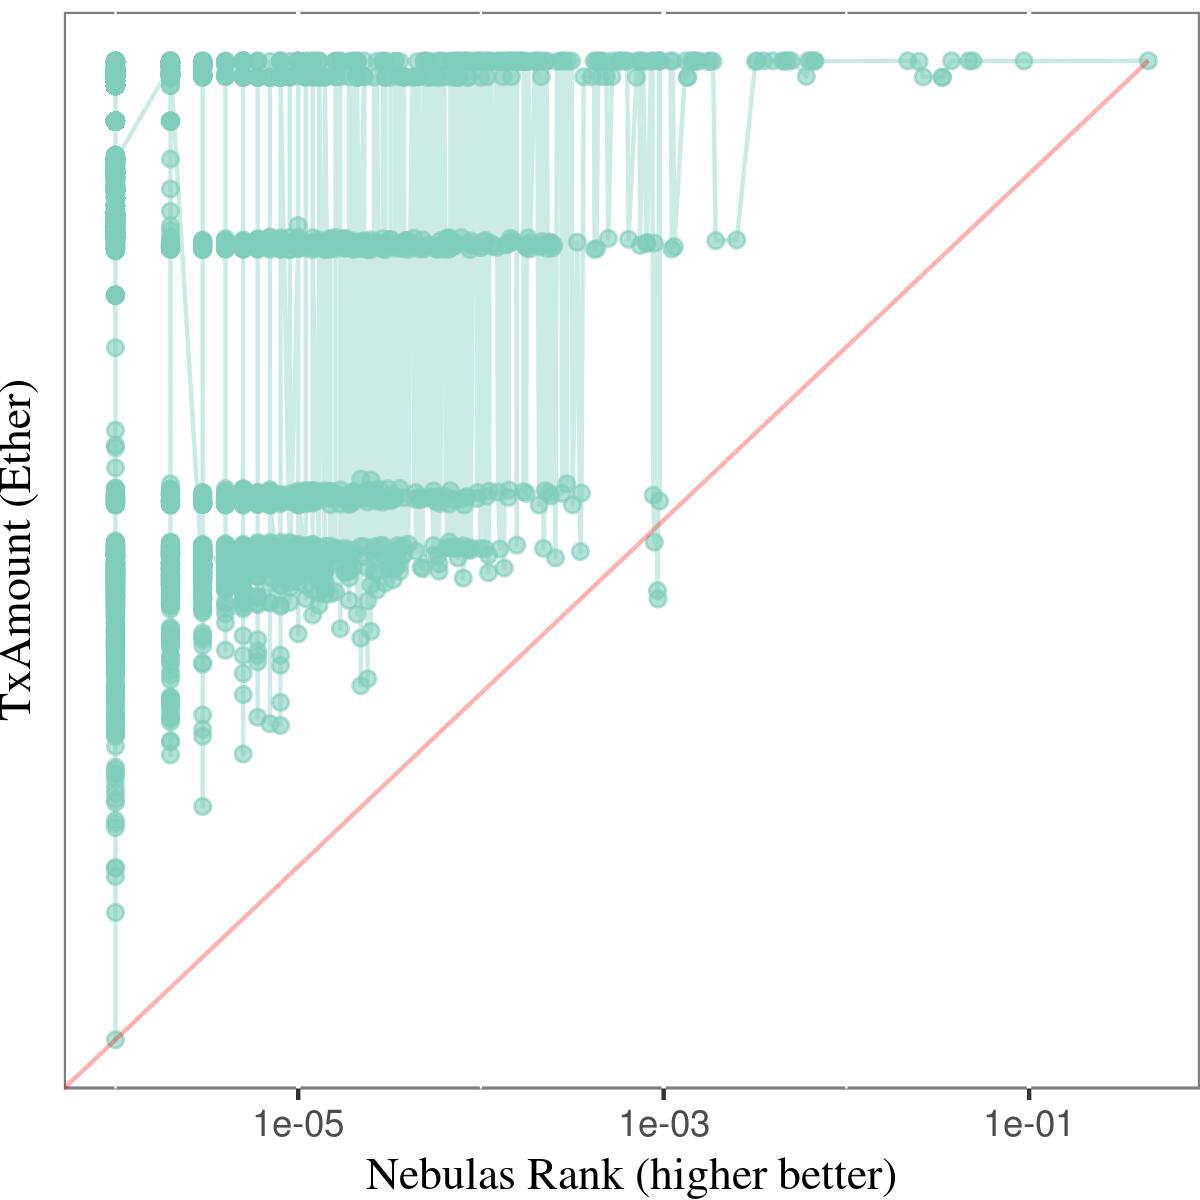
\includegraphics[width=0.50\textwidth]{figs/MAY_lr.png}
	\caption{Nebulas Rank v.s. Transaction Amount \small{X-axis represents Rank Value, and Y-axis represents Transaction Amount, both in logarithmic form.  The diagonal line represents that transaction amount and rank value is directly proportional. A good algorithm should make the data points fall as little as possible in the lower right of the diagonal line, to avoid nodes with low transaction throughput to get high rank.}}\label{fig:nrio}
\end{figure}

According to the above simple analysis, it can be deduced that the first three types of manipulation can be filtered effectively by specific methods. Therefore finally, we just need to simulate the last type and observe the resistance effect. The attacker chooses one authoritative Exchange node to create loop transfers for $X$ times. Every loop transfer contains 2 phases: first the attacker transfers $Y$ Ether to the Exchange through some newly created temporary address; then the attacker retrieves its money back from the Exchange through another address. The attacking topology and process is demonstrated in \reffig{fig:loop}. This type of attack exploits the fact that an Exchange service is willing to establish links with any nodes at a very low cost. Although normal nodes can also transfer with Exchange nodes frequently, but such attacking activities do not improve effective money liquidity and should be distinguished from normal activities.
\begin{figure}[!ht]
	\centering
	%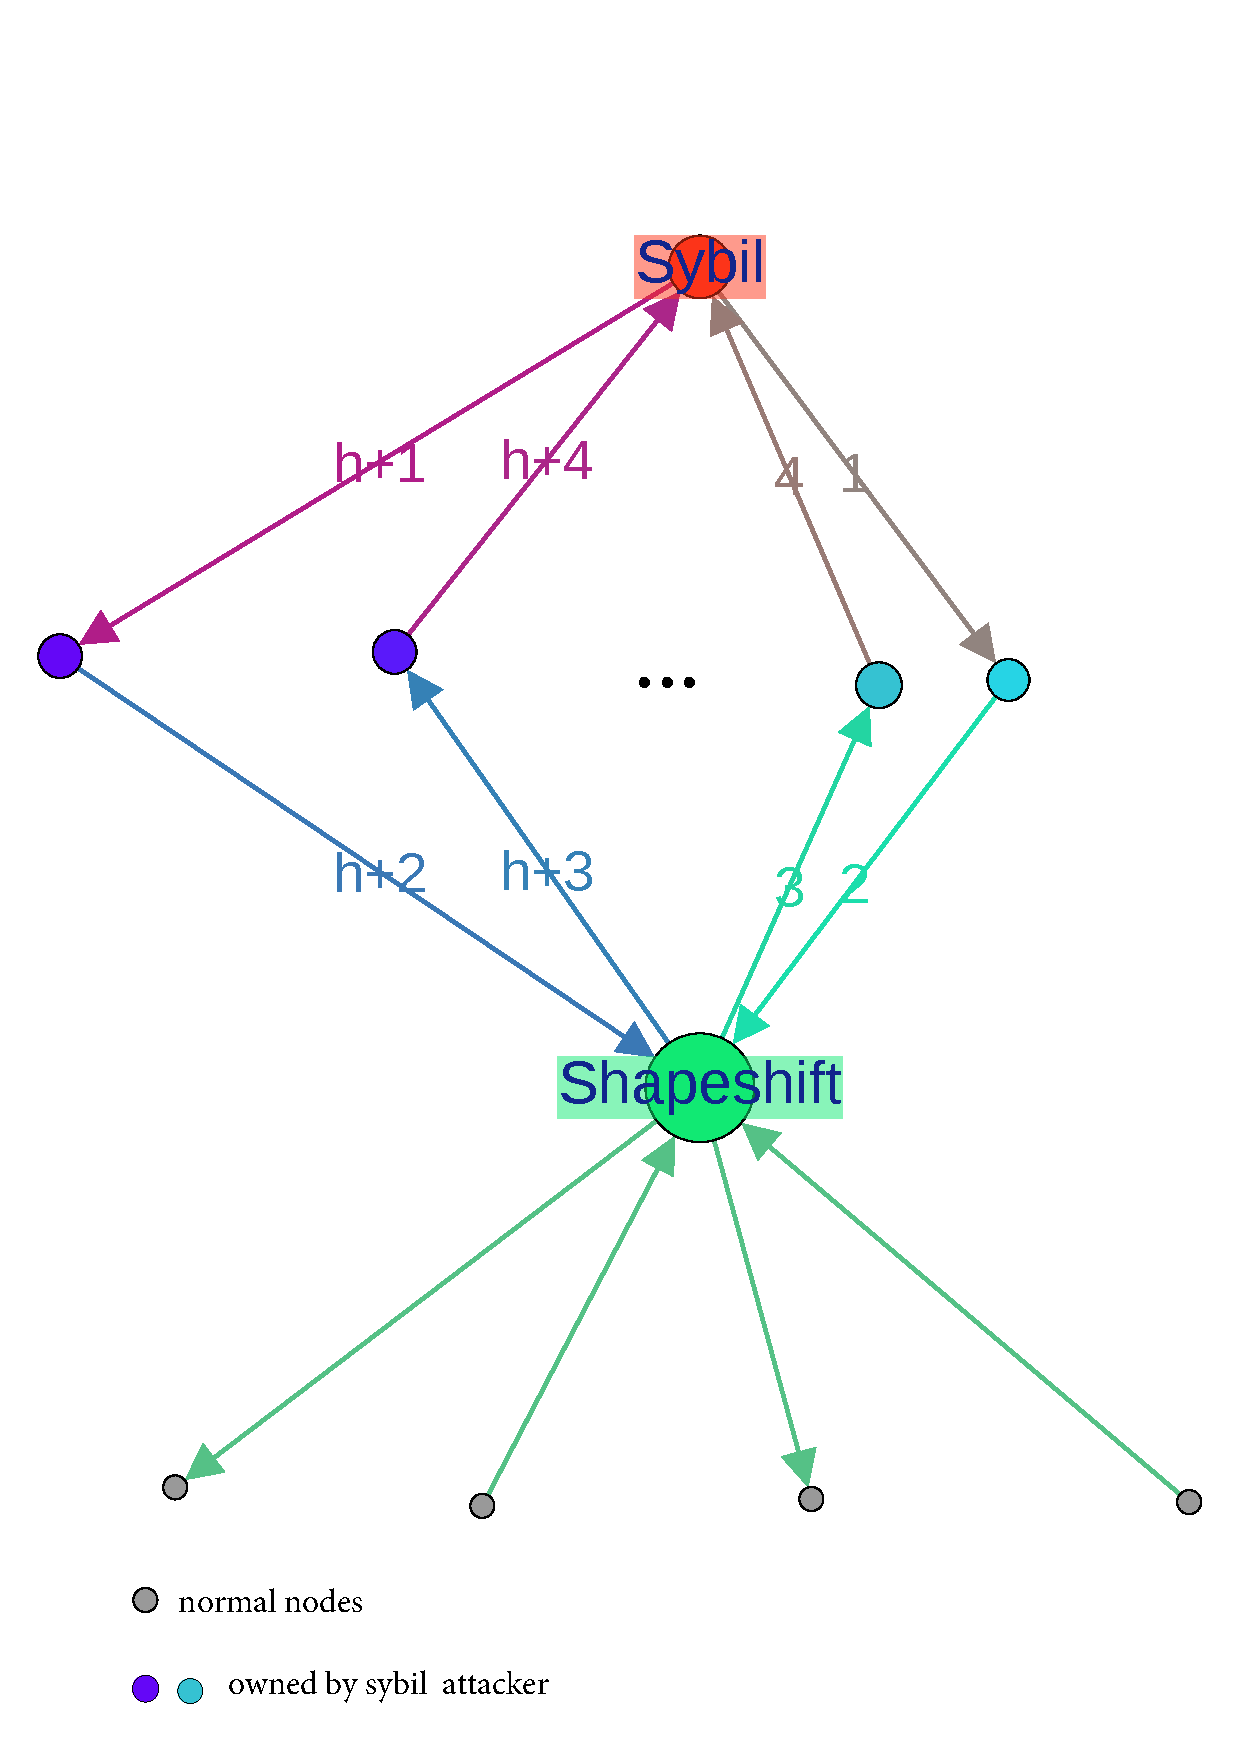
\includegraphics[width=0.35\textwidth]{figs/attack.pdf}
  \begin{tikzpicture}
  \pgfmathsetmacro{\YMD}{2}
  \pgfmathsetmacro{\XMD}{1.5}
\tikzset{
  hnode/.style={draw, circle, on grid, align=center, minimum height=2ex},
  base/.style={draw, circle, on grid, align=center, minimum height=4ex},
  sybil/.style={draw, circle, on grid, align=center, minimum height=4ex, fill=blue!20},
  normal/.style={draw, circle, on grid, align=center, minimum height=1ex, fill=gray!20},
  coord/.style={coordinate, on grid, node distance=6mm and 25mm},
}
%
\tikzset{>=stealth',
  every join/.style={->}, very thick}

       \node [base, fill=green!=20] (ss) at (0, 0) {} node[right
       = 1ex of ss] {Shapeshfit};

       \node (dot) at ($(ss.north) + (0, \YMD)$) {...};

       \node [sybil] (sy) at ($(dot.north) + (0, \YMD)$) {} node[right=1ex of
       sy]{Sybil};

       \node [hnode, fill=brown!50] (hh4) at($(dot.west) + (-\XMD, 0)$){};
       \node [hnode, fill=brown!50] (hh1) at ($(hh4.west) + (-\XMD, 0)$){};

       \node [hnode, fill=cyan!20] (h4) at ($(dot.east) + (\XMD, 0)$){};
       \node [hnode, fill=cyan!20] (h1) at ($(h4.east) + (\XMD, 0)$){} node
       [right = 1ex of h1]{owned by sybil attacker};

       \node [coord] (c) at($(ss.south) + (0, -\YMD)$) {};

       \node [normal] (n2) at ($(c.west) + (-\XMD, 0)$){};
       \node [normal] (n1) at ($(n2.west) + (-\XMD, 0)$){};
       \node [normal] (n3) at ($(c.east) + (\XMD, 0)$){};
       \node [normal] (n4) at ($(n3.east) + (\XMD, 0)$){} node [right=1ex of
       n4] {normal nodes};

       \draw[->, color=red] (sy) -- (hh1) node [midway, left]{h+1};
       \draw[->, color=red] (hh4) -- (sy) node [midway, right]{h+4};
       \draw[->, color=olive] (h4) -- (sy) node [midway, left]{4};
       \draw[->, color=olive] (sy) -- (h1) node [midway, right]{1};

       \draw[->, color=red] (hh1) -- (ss) node [midway, left]{h+2};
       \draw[->, color=red] (ss) -- (hh4) node [midway, right]{h+3};
       \draw[->, color=olive] (ss) -- (h4) node [midway, left] {3};
       \draw[->, color=olive] (h1) -- (ss) node [midway, right]{2};

       \draw[->] (ss) -- (n1);
       \draw[->] (n2) -- (ss);
       \draw[->] (ss) -- (n3);
       \draw[->] (n4) -- (ss);

\end{tikzpicture}

	\caption{Schematic of Loop Attack Utilizing Exchange Address \small{The first and $h$-st loop attacks are shown in the figure. The selected authoritative Exchange node is Shapeshift; Edge label indicates temporal sequence; The transfer amount between nodes controlled by Sybil attacker and Shapeshift node is $Y$Ether; There are $X$ loop transfers during the manipulation.}}\label{fig:loop}
\end{figure}

We choose Shapeshift(0x70faa28a6b8d6829a4b1e649d26ec9a2a39ba413) as the authoritative Exchange address. The results is shown in \reffig{fig:antiManipulation}: 1) As is shown in \reffig{subfig:deposit}, with the attacker investing more capital, no algorithm is able to prevent the attacker's rank from being better, while the transaction graph defined in \refsec{subsec:txg} reduces the attacking effect. \textbf{Nebulas Rank} can not only prefer nodes with high transaction throughput, but also resist manipulation to some extent; 2) As is shown in \reffig{subfig:times}, with the attacker making more loop transfers, the transaction graph defined at \refsec{subsec:txg} can let the attacker's rank be worse. The reason is that such transaction graph considers factors like coinage and encouragement value. Meanwhile, \textbf{Nebulas Rank} could strengthen these factors, bringing more resistance against manipulation.

\begin{figure}[htbp]
	\centering
	\begin{subfigure}{\linewidth}
		\centering
		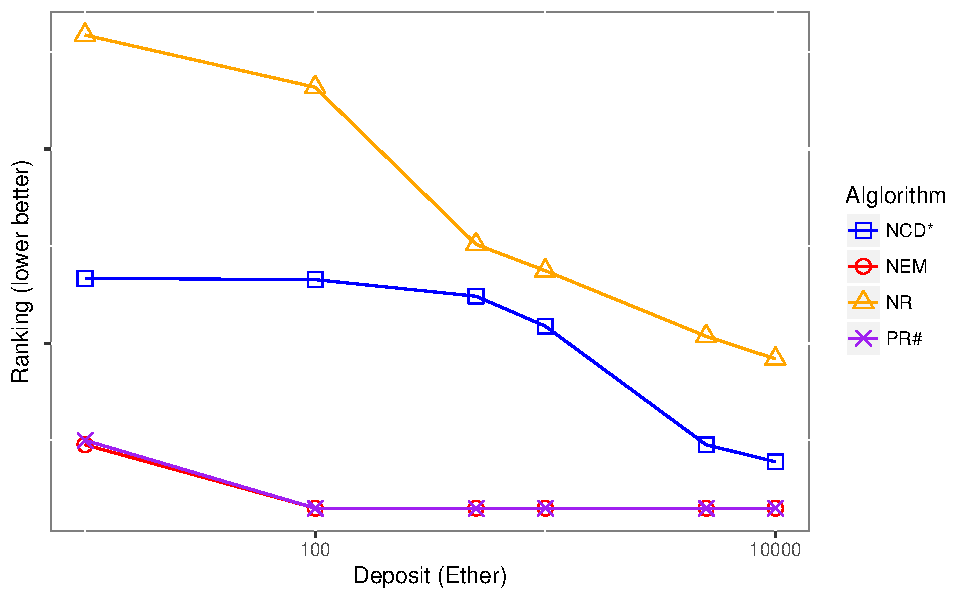
\includegraphics[width=0.7\textwidth]{figs/AttackDeposit.pdf}
		\caption{The effect of attacker's capital size on attacker's rank, with the number of loop transfers is fixed as $5,000$. \small{(All axises are in logarithmic form)}}
		\label{subfig:deposit}
	\end{subfigure}
	
	\begin{subfigure}{\linewidth}
	    \centering
		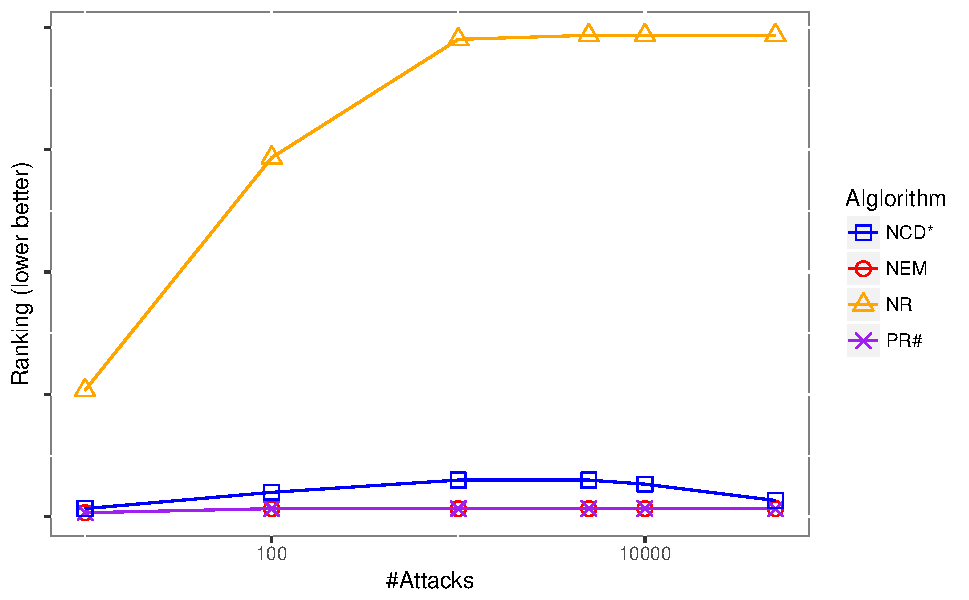
\includegraphics[width=0.7\textwidth]{figs/AttackTimes.pdf} 
		\caption{The effect of number of loop transfers on the attacker's rank, with attacker's capital fixed as $\Xi5000$ \small{(All axises are in logarithmic form)}}\label{subfig:times}
	\end{subfigure}

	\caption{Resistance against manipulation} \label{fig:antiManipulation}
	\caption*{\footnotesize{The attacking method is shown as \reffig{fig:loop}; x-axis represents attacker's capital; y-axis represents attacker's ranking order (larger ranking order means the attacker fails to get better score, indicating higher resistance ability of the algorithm)  \\
	NR:The transaction graph is defined at \refsec{subsec:txg}, and ranking algorithm is described at \refsec{subsec:leaderrank}; \\
	%PR$^*$: The transaction graph is defined at \refsec{subsec:txg}, PageRank algorithm;\\ 
	NCD$^*$: The transaction graph is defined at \refsec{subsec:txg}, with NCDawareRank algorithm; \\
	NEM:The transaction graph is introduced by \cite{nem}, with NCDawareRank\\ 
	PR$^{\#}$: The transaction graph is introduced by \cite{nem},with PageRank algorithm\\ 
	The damping factor of PageRank is 0.15; The clustering algorithm used by NCDawareRank is pscan\cite{chang2017mathsf}, $\eta=0.75$, $\mu=0.1$}}
\end{figure}

\subsection{Related Works} \label{subsec:related}

Centrality, the core ranking index, is a most studied concept in network science since decades ago\cite{newman2010networks}. There are a body of literatures introducing various centralities, including degree centrality\cite{freeman1979set}, eigenvector centrality\cite{bonacich1972factoring}, Katz centrality\cite{katz1953new}, closeness centrality\cite{sabidussi1966centrality}, betweenness centrality\cite{freeman1977set}\cite{freeman1978centrality}\cite{freeman1991centrality}\cite{noh2004random}\cite{newman2005measure}, PageRank\cite{Brin2010}, HITS\cite{kleinberg1999authoritative}, SALSA\cite{Science2001}, etc. Besides, there are some fundamental works trying to clearly classify and review these measurements by a unified framework\cite{Borgatti2005}\cite{Borgatti2006}\cite{Lu2016}. When designing \textbf{Nebulas Rank}, before proper centrality is adopted, first we need to consider the property of graph. Blockchain transaction graph's scenario is most similar to the money exchange flow network mentioned in \cite{Borgatti2005}. But the related algorithms mentioned by their work, such as flow betweenness centrality\cite{freeman1991centrality} and random-walk betweenness centrality (aka. current betweenness centrality)\cite{newman2005measure}, are compute intensive and do not satisfy the property of "computable" with the large scale of Blockchain transaction graph.

Since Bitcoin\cite{Nakamoto2008} system released in 2009, researchers have done some statistical and empirical analysis on Bitcoin's transaction graph\cite{Ron}\cite{Haslhofer}\cite{NielKondor2014}\cite{Baumann2014}, and some use the transaction graph structure to discuss anonymity in Bitcoin\cite{Meiklejohn2013}\cite{Ober2013}\cite{pham2016anomaly}\cite{Fleder2015}\cite{Ferrin2015}. After other cryptocurrencies emerged and become popular, transaction graph analysis is conducted for more blockchains\cite{Chang2017}\cite{Anderson2016}. \textbf{Nebulas Rank} adopts their transaction graph concept, i.e. Entity Graph in \cite{Tschorsch2015}, with minor revisions. That is, each account, or set of accounts belonging to the same people, is mapped as a node, and each directed edge represents the intensity of transferring between two accounts. Actually before blockchain system like Bitcoin was invented, scientists have tried to study some financial networks among banks and global trading entities\cite{propper2008towards}\cite{Boss2004}\cite{Serrano2007}\cite{Bech2008}\cite{Fagiolo2009}\cite{Morten2006}\cite{Boss2004a}\cite{Krempel2002}\cite{Serrano2003}. Comparing with blockchain transaction graph, these early studied finical networks are defined not only by transferring activities, but also by extra information such as loan. Moreover, the scale of these networks is much smaller. To conclude, there is rarely research work proposing custom ranking method for large scale transaction graph, especially blockchain transaction graph.

The most relevant work with \textbf{Nebulas Rank} is NEM\cite{nem}'s Proof-of-Importance scheme. It adopts NCDawareRank\cite{Nikolakopoulos2013}, which exploits the clustering effect of network topology, as the ranking algorithm, with clustering algorithm based on SCAN algorithm\cite{xu2007scan}\cite{shiokawa2015scan}\cite{chang2017mathsf}. Although community structure does exist in transaction graph and should be helpful to handle with spam nodes, it does not guarantee that all nodes in Blockchain world controlled by one entity in the real world are mapped into one cluster, which leads to large room for manipulation. Besides, \textcite{Fleder2015} uses PageRank\cite{Brin2010}\cite{page1999pagerank} as an assisting metric to discover interesting addresses and analyze their activities. However, their work does not provide an automated framework to identify important nodes. Instead, it still relies on subjective analysis, which does not match \textbf{Nebulas Rank}'s context. The algorithm we choose is LeaderRank\cite{Chen2013}\cite{Li2014}. It is a simple yet effective variant of PageRank\cite{Brin2010}\cite{page1999pagerank}. In PageRank, every node is assigned with identical teleportation parameter, while LeaderRank adds a ground node, assigning different teleportation parameters for each node. The weighing scheme of \textbf{Nebulas Rank} is partly from \textcite{Li2014}'s design, which allows nodes with more in-degree to be more likely visited by teleportation. Adopting LeaderRank algorithm could yield results more suitable for the scenario of Blockchain.

